\section{Simulación de Vuelo}

La dinámica y trayectoria del cohete PDA STARS se verificaron mediante simulaciones numéricas en seis grados de libertad en OpenRocket, utilizando la curva de empuje certificada por NAR/TRA para el motor oficial Estes F15-4 (impulso total 49,6 N·s, empuje medio 14,8 N, tiempo de combustión nominal 3,4 s, retardo de eyección 4,0 s) y condiciones atmosféricas locales estándar (densidad del aire $\rho = 1,05\text{ kg/m}^3$ a 1700 msnm, viento cruzado de hasta 3,5 m/s).

\begin{figure}[H]
\centering
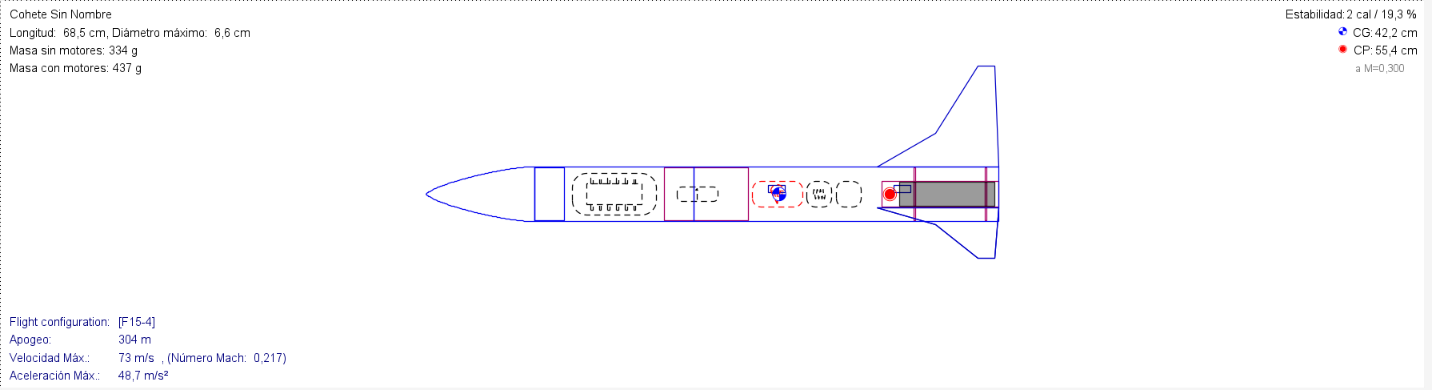
\includegraphics[width=0.85\linewidth]{vista_lateral_cohete.png}
\caption{Vista lateral y configuración de análisis aerodinámico del cohete PDA STARS.}
\label{fig:vista_lateral}
\end{figure}

\subsection{Resultados Numéricos Consolidados}
Los datos extraídos directamente de la simulación oficial (\texttt{simulacion\_stellaris.csv}) y el modelo \texttt{211\_PDASTARS\_Diseño.ork} confirman los siguientes parámetros de vuelo:

\begin{table}[H]
\centering
\small
\begin{tabularx}{\linewidth}{Xccp{4.5cm}}
\toprule
\rowcolor{navyiejaga!15}
\textbf{Parámetro de Vuelo} & \textbf{Valor Simulado} & \textbf{Límite / Meta CCCD} & \textbf{Estado de Cumplimiento} \\
\midrule
\textbf{Velocidad en salida de varilla ($1,5\text{ m}$)} & 10,70 m/s (38,5 km/h) & $\ge 10,0\text{ m/s}$ & Cumple (control aerodinámico inmediato) \\
\rowcolor{grisclaro}
\textbf{Aceleración vertical máxima} & 48,68 m/s² (4,96 G) & $< 15\text{ G}$ & Cumple (cargas tolerables en Kraft/epoxi) \\
\textbf{Velocidad máxima de ascenso} & 73,01 m/s (Mach 0,217) & Subsonico ($< 0,3$) & Cumple (baja resistencia compresible) \\
\rowcolor{grisclaro}
\textbf{Tiempo hasta el apogeo} & 8,90 s & Nominal 8--10 s & Cumple (trayectoria ascendente estable) \\
\textbf{Apogeo máximo alcanzado} & \textbf{304,22 m} & \textbf{300,0 m} & \textbf{Cumple} (desviación mínima de $+1,4\%$) \\
\rowcolor{grisclaro}
\textbf{Velocidad al abrir paracaídas} & 17,86 m/s (a los 8,5 s) & $< 25\text{ m/s}$ & Cumple (eyección segura cerca al apogeo) \\
\textbf{Velocidad terminal de descenso} & \textbf{8,00 m/s} ($7,998\text{ m/s}$) & $6,0\text{ -- }9,0\text{ m/s}$ & Cumple (aterrizaje sin impacto estructural) \\
\rowcolor{grisclaro}
\textbf{Duración total del vuelo} & \textbf{47,86 s} & \textbf{40 a 50 s (Motor F)} & \textbf{Cumple} (centrado en la ventana oficial) \\
\textbf{Deriva radial máxima} & 125,0 m & $< 250,0\text{ m}$ & Cumple (recuperación en radio seguro) \\
\bottomrule
\end{tabularx}
\caption{Consolidado de parámetros de ingeniería de la simulación de vuelo oficial.}
\label{tab:resumen_simulacion}
\end{table}

\begin{figure}[H]
\centering
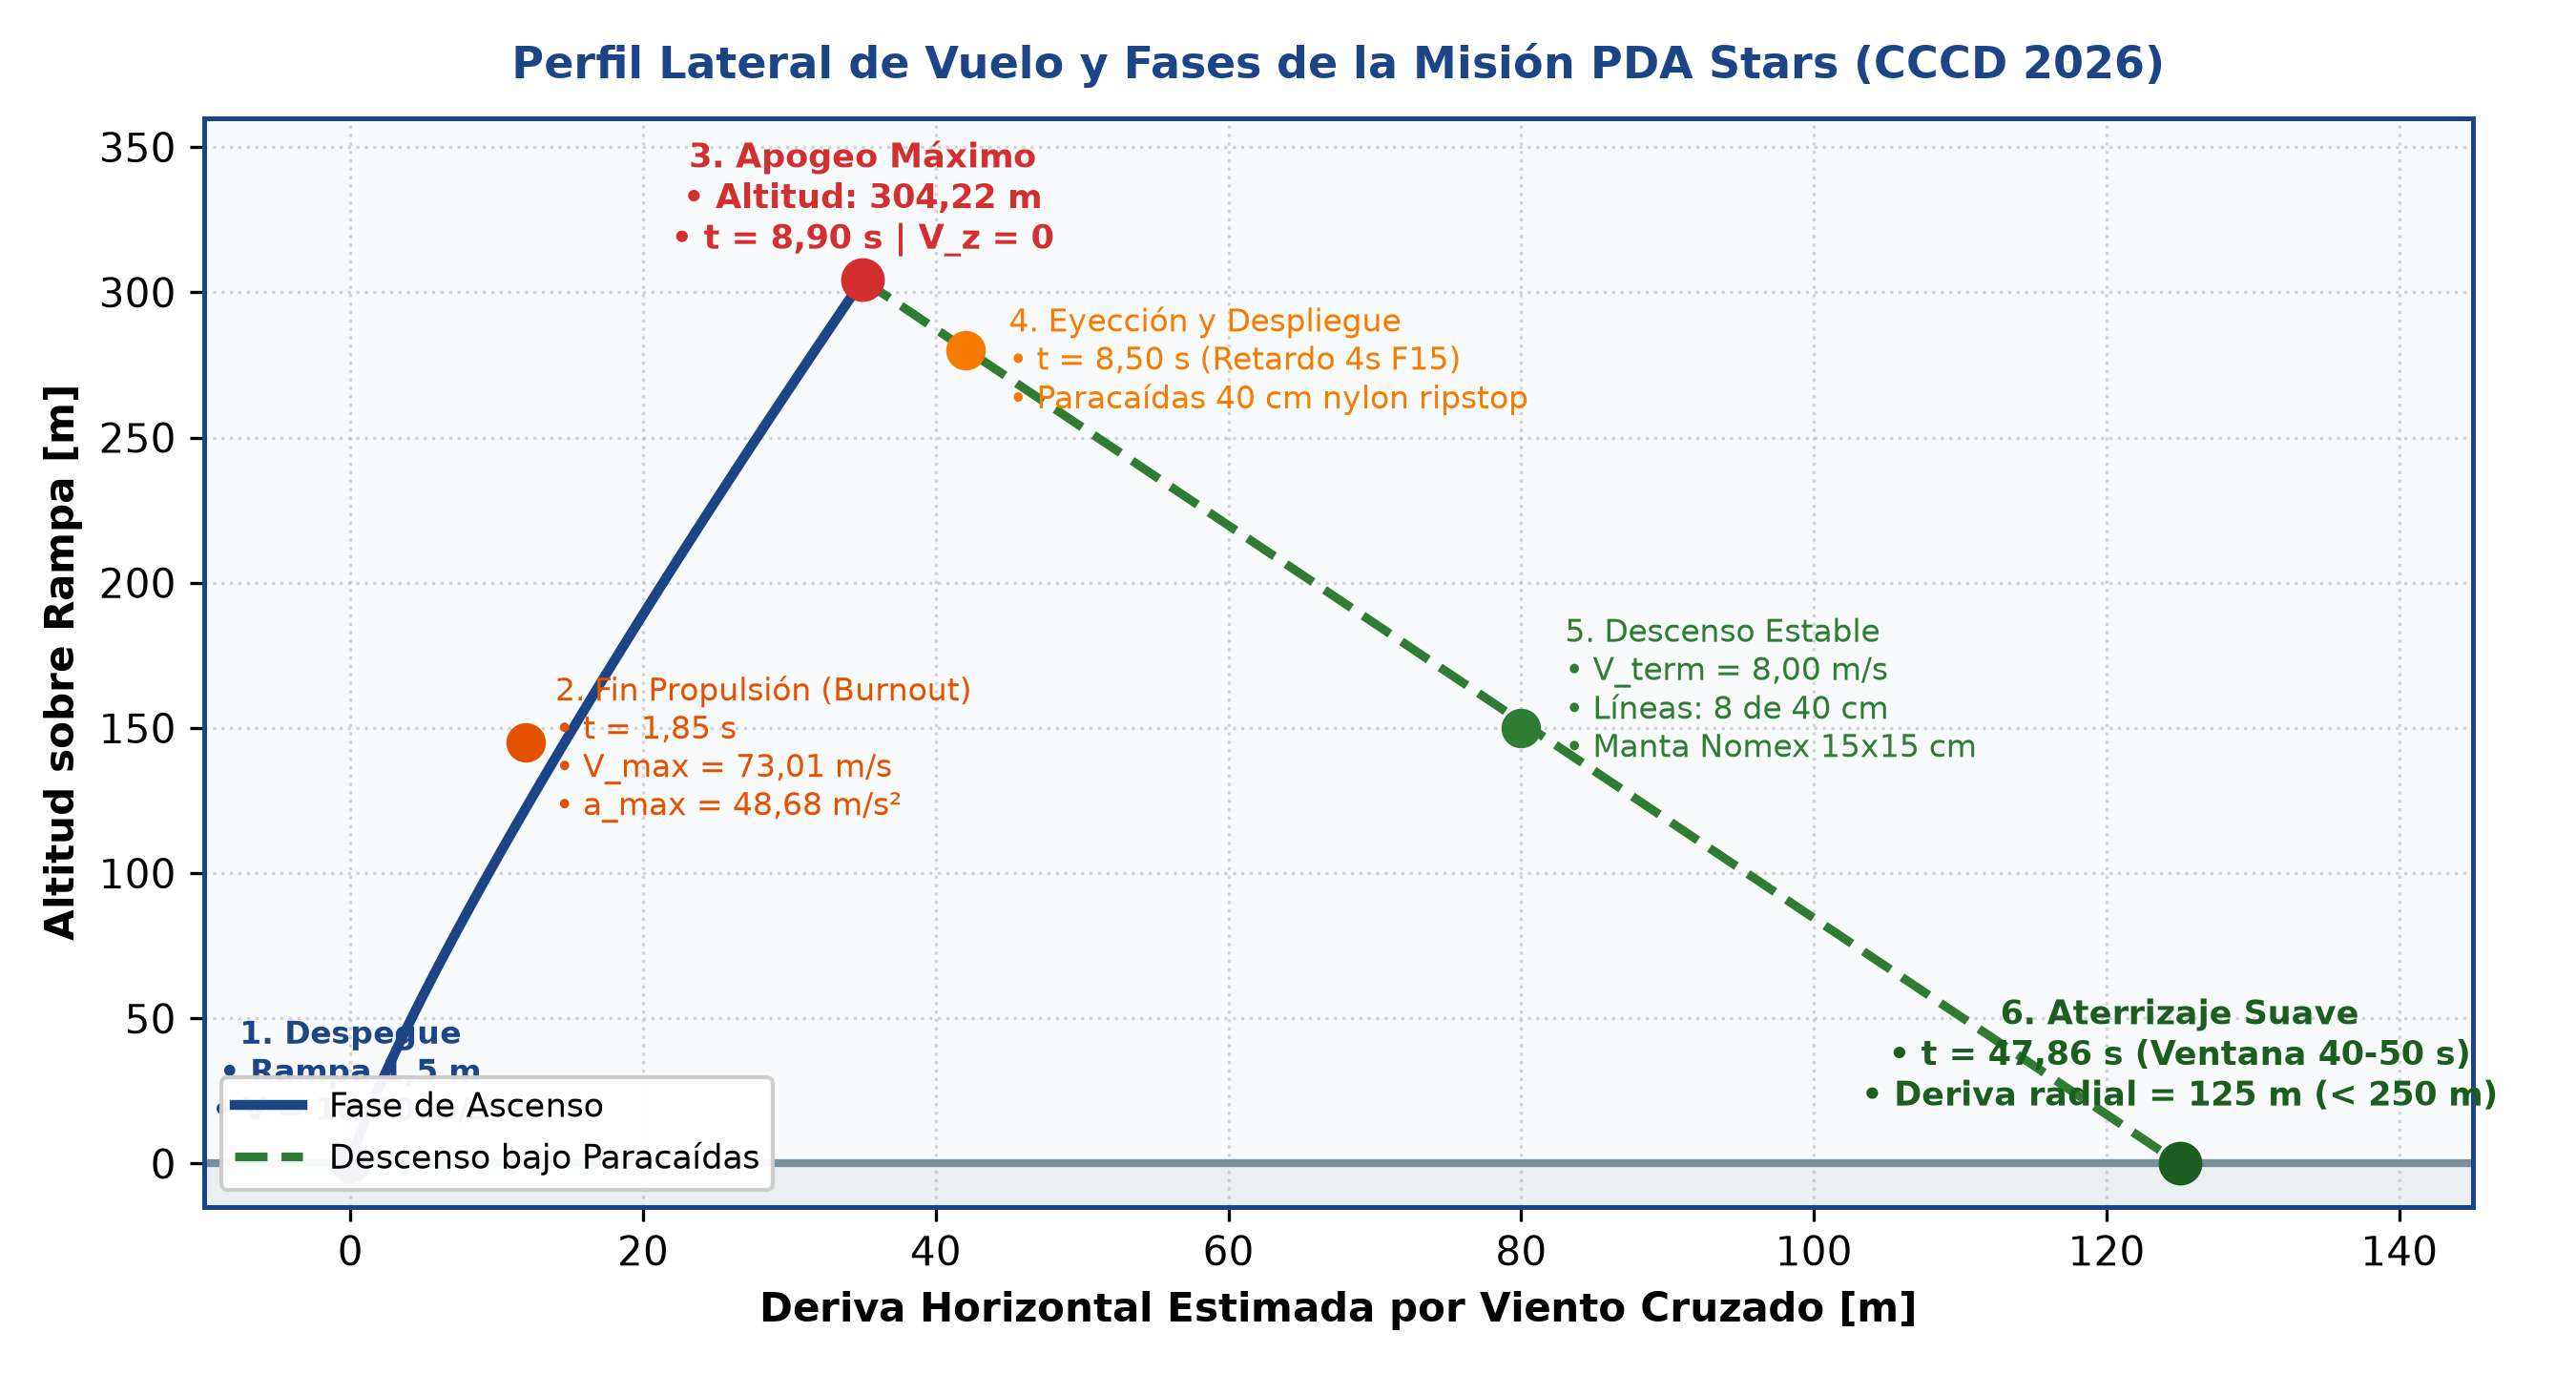
\includegraphics[width=0.95\linewidth]{fig_perfil_lateral_vuelo.png}
\caption{Perfil lateral de vuelo y eventos secuenciales de la misión PDA STARS.}
\label{fig:perfil_vuelo}
\end{figure}

\subsection{Curvas Dinámicas de Trayectoria}
A continuación se presentan las curvas temporales de altitud, velocidad y aceleración obtenidas del modelo validado:

\begin{figure}[H]
\centering
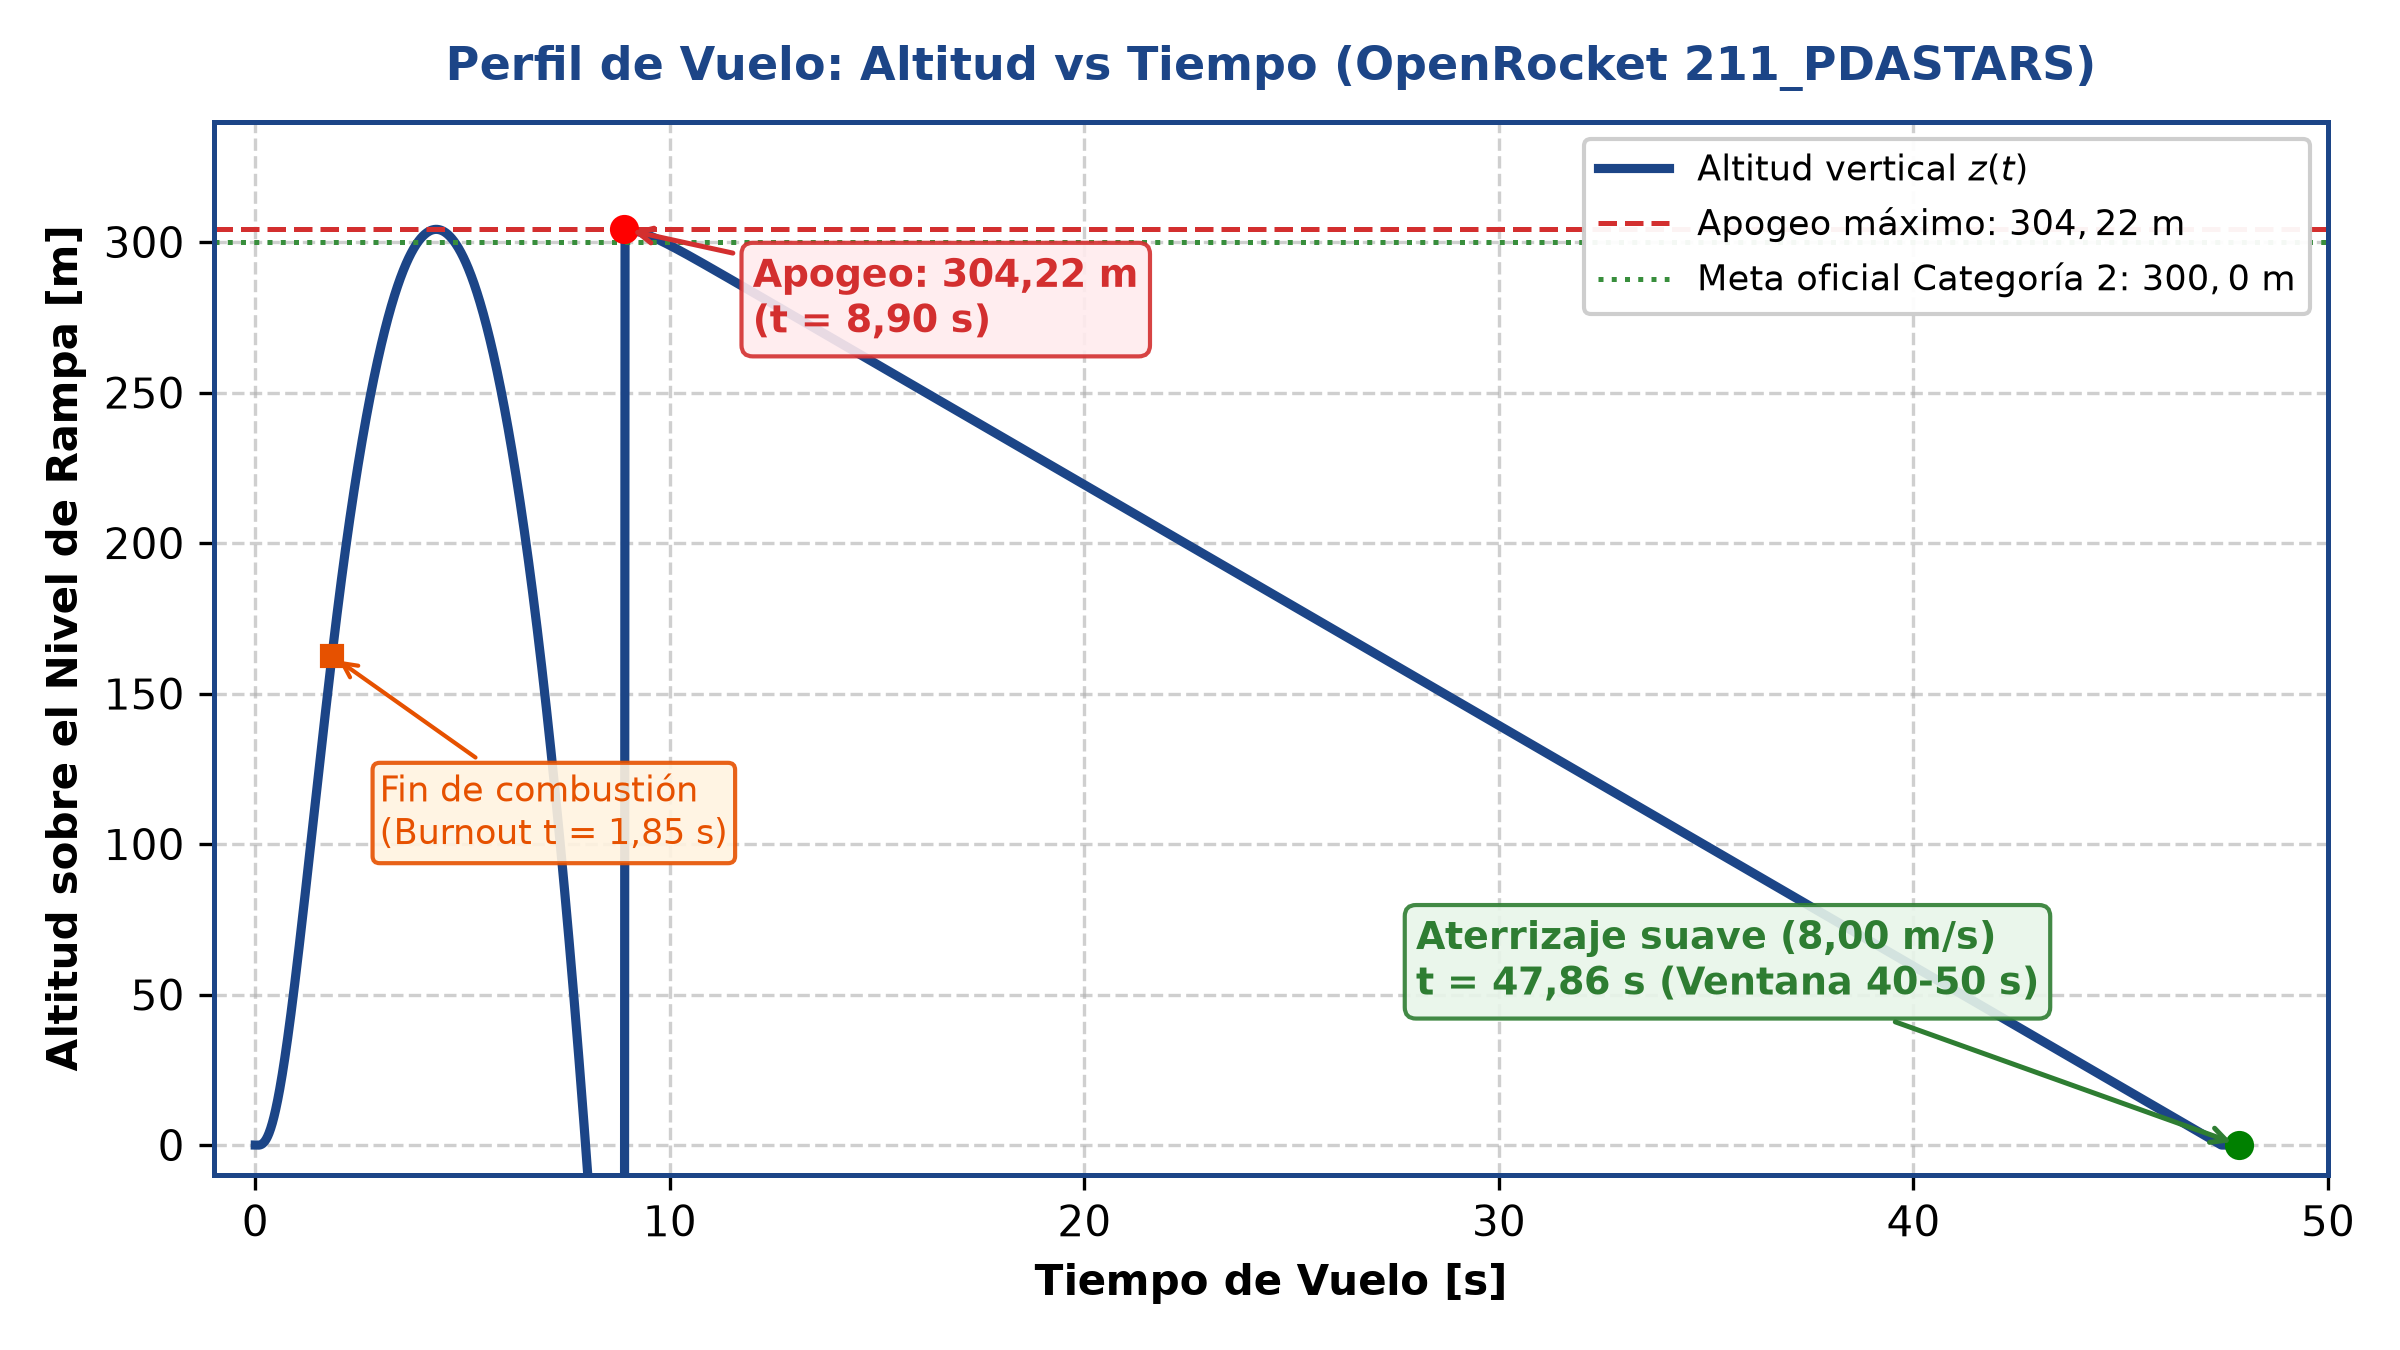
\includegraphics[width=0.9\linewidth]{fig_altitud_tiempo.png}
\caption{Curva de altitud vs tiempo (Apogeo máximo de $304,22\text{ m}$ y tiempo total de $47,86\text{ s}$).}
\label{fig:altitud_tiempo}
\end{figure}

\begin{figure}[H]
\centering
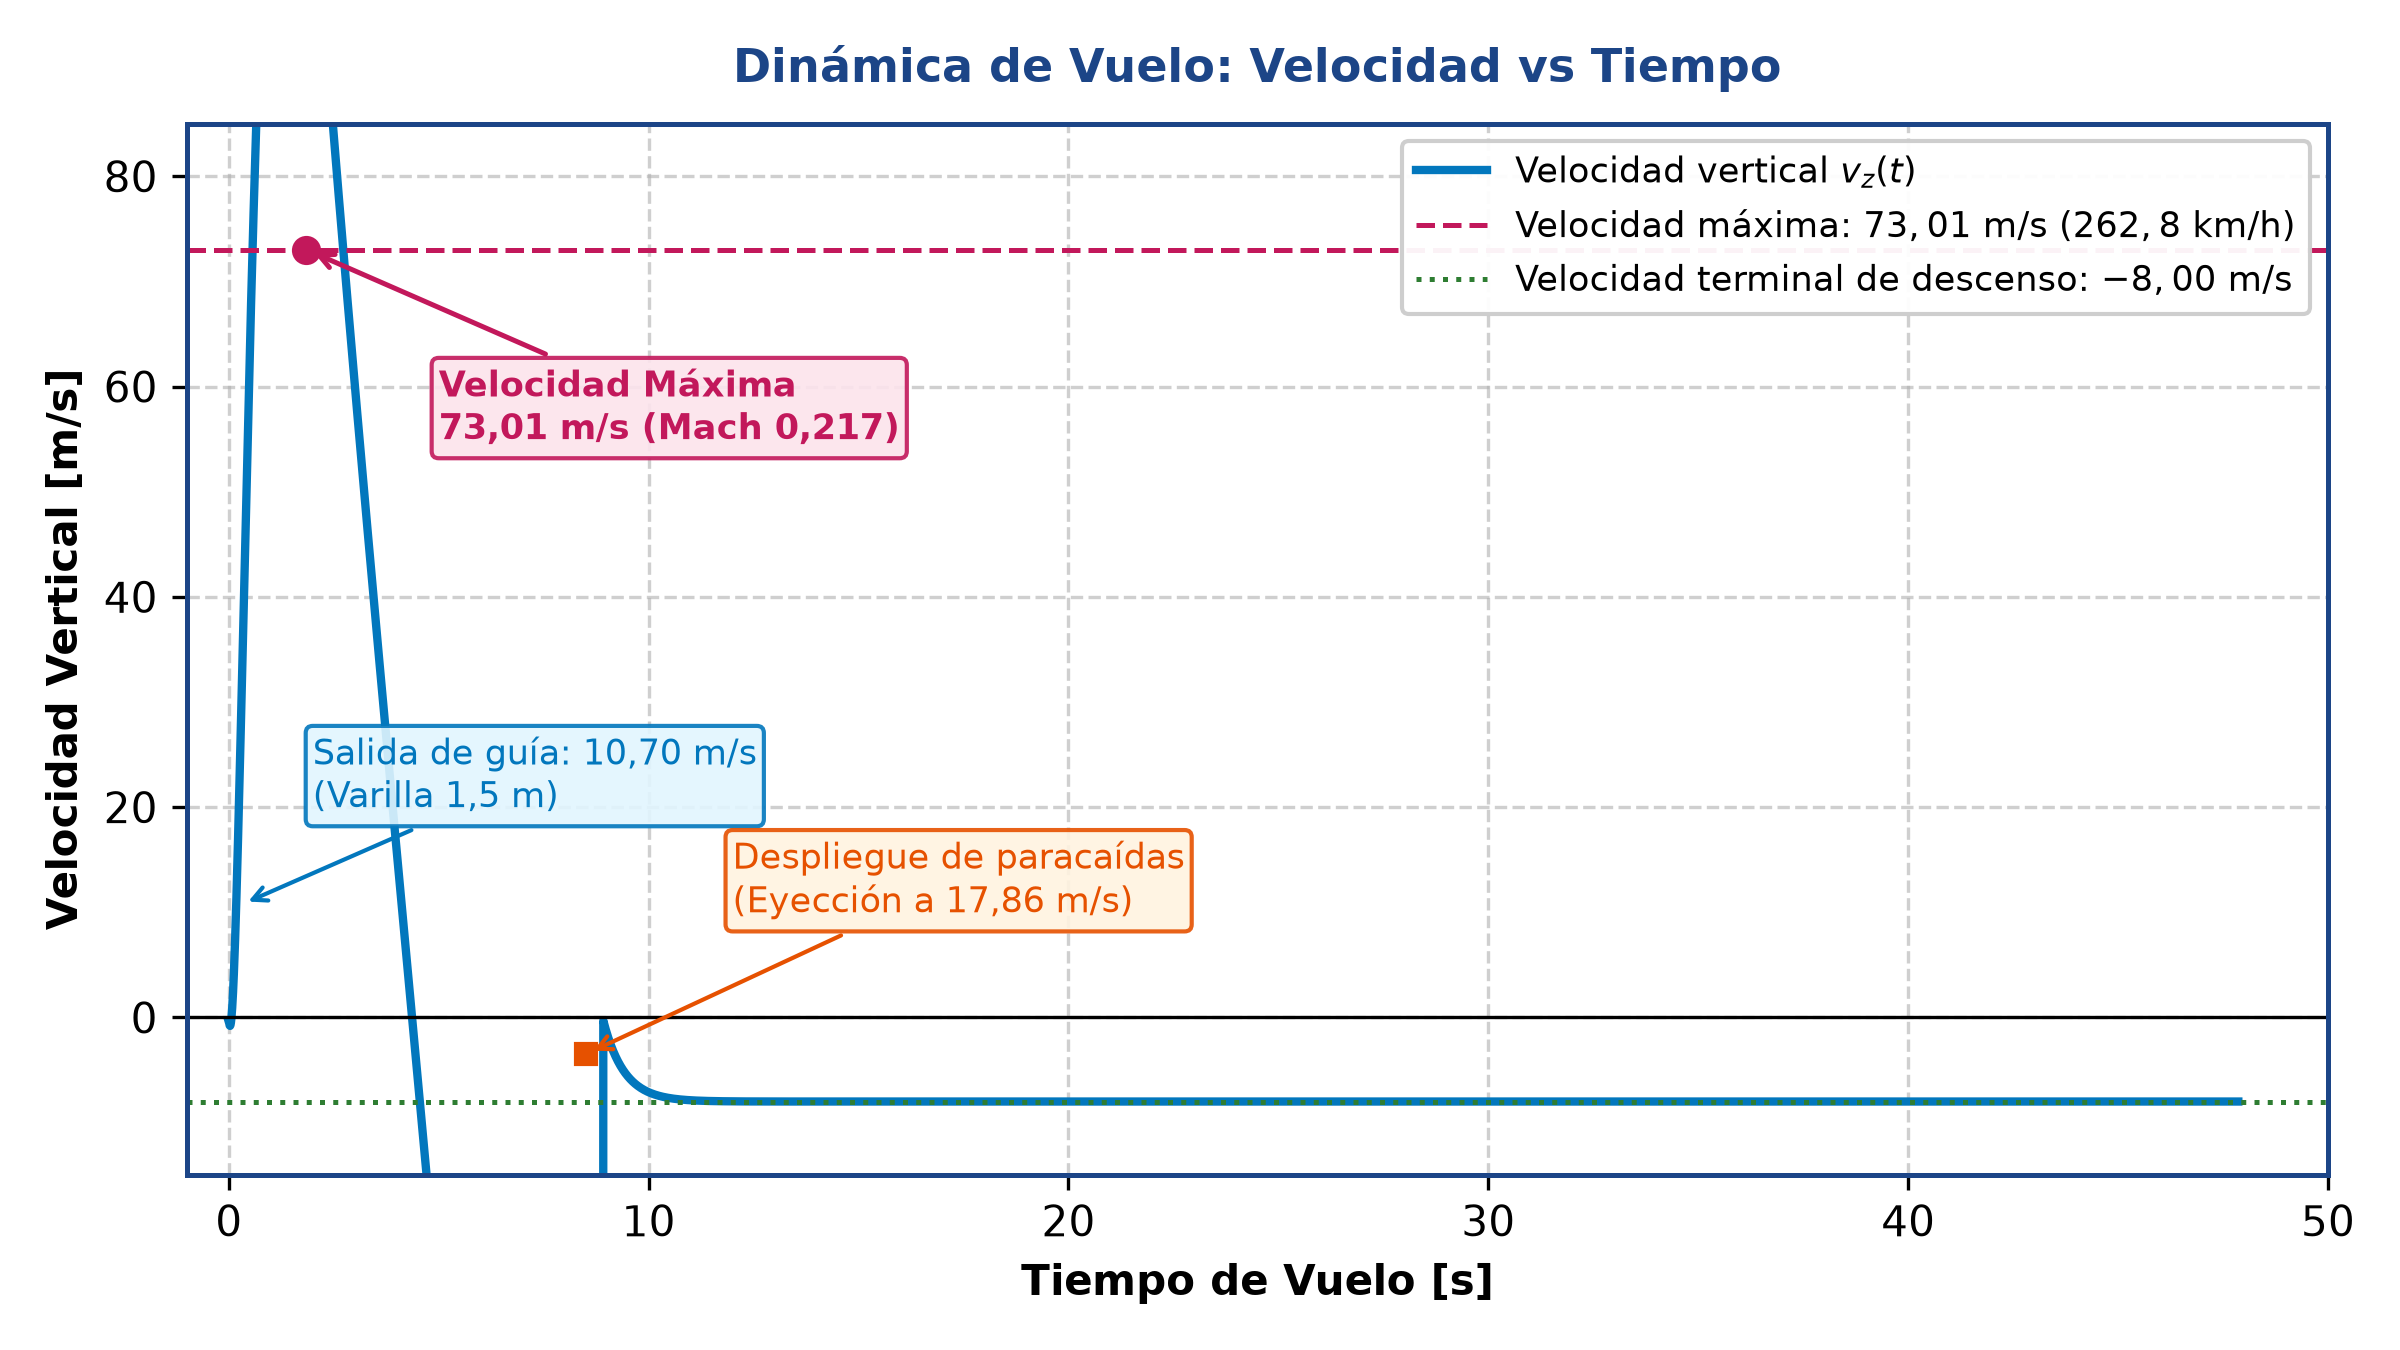
\includegraphics[width=0.9\linewidth]{fig_velocidad_tiempo.png}
\caption{Curva de velocidad vertical vs tiempo ($v_{max} = 73,01\text{ m/s}$, $v_{term} = 8,00\text{ m/s}$).}
\label{fig:velocidad_tiempo}
\end{figure}

\begin{figure}[H]
\centering
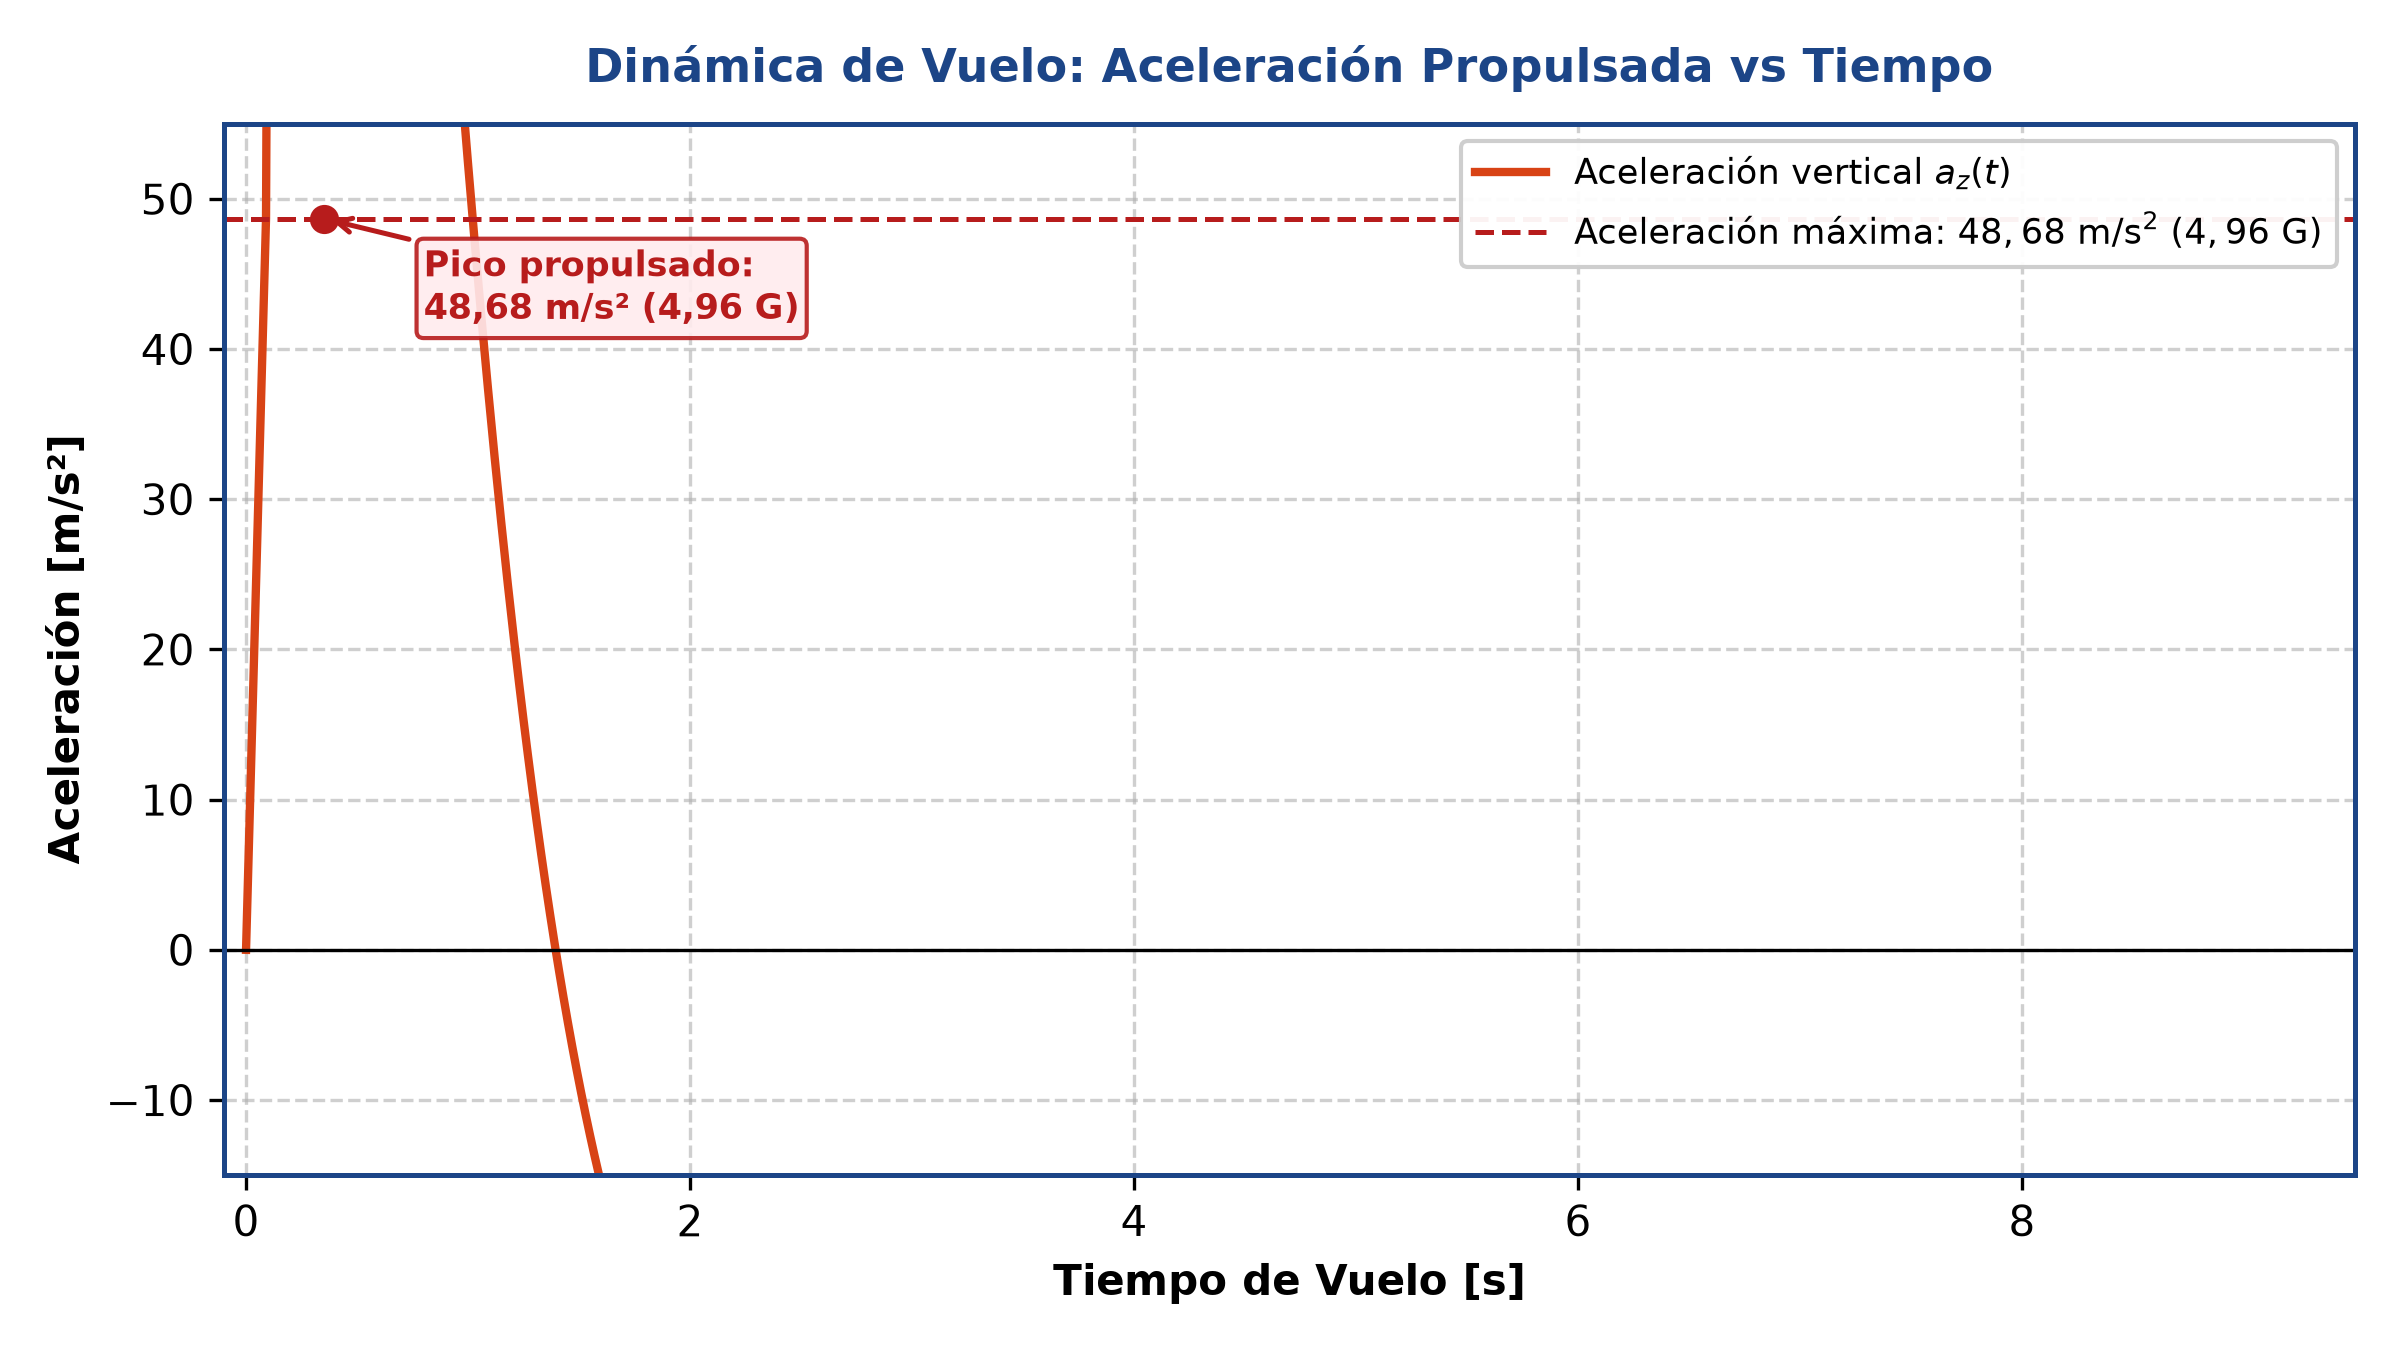
\includegraphics[width=0.9\linewidth]{fig_aceleracion_tiempo.png}
\caption{Curva de aceleración propulsada vs tiempo (pico máximo de $48,68\text{ m/s}^2$ / $4,96\text{ G}$).}
\label{fig:aceleracion_tiempo}
\end{figure}
